% \section{Mechanism of ChatGPT-powered Chatbot}
% % \KZ{I think this section can go into the main text. The prompt design part
% % turns out to be not so important and can be shortened.}
% We utilize the chat model\footnote{\url{https://platform.openai.com/docs/guides/chat/}} developed by OpenAI to build our chatbots. 
% This model operates by taking a sequence of \textit{messages} as input, and returns a model-generated response. 
% % Each \textit{message} in the input sequence is composed of two parts: a role (either ``system'', ``user'', or ``assistant'') and content (the actual message itself). In most cases, a conversation begins with a system message that establishes the behavior of the assistant, followed by alternating user and assistant messages as the dialogue progresses. 
% As Figure \ref{fig:process} shows, at each turn, we combine the system message and the ongoing conversation history with alternating user and assistant messages into a sequence and feed them into the ChatGPT language model. The resulting output is the Chatbot's response to the user's input.
% \begin{figure}[th]
% 	\centering
% 	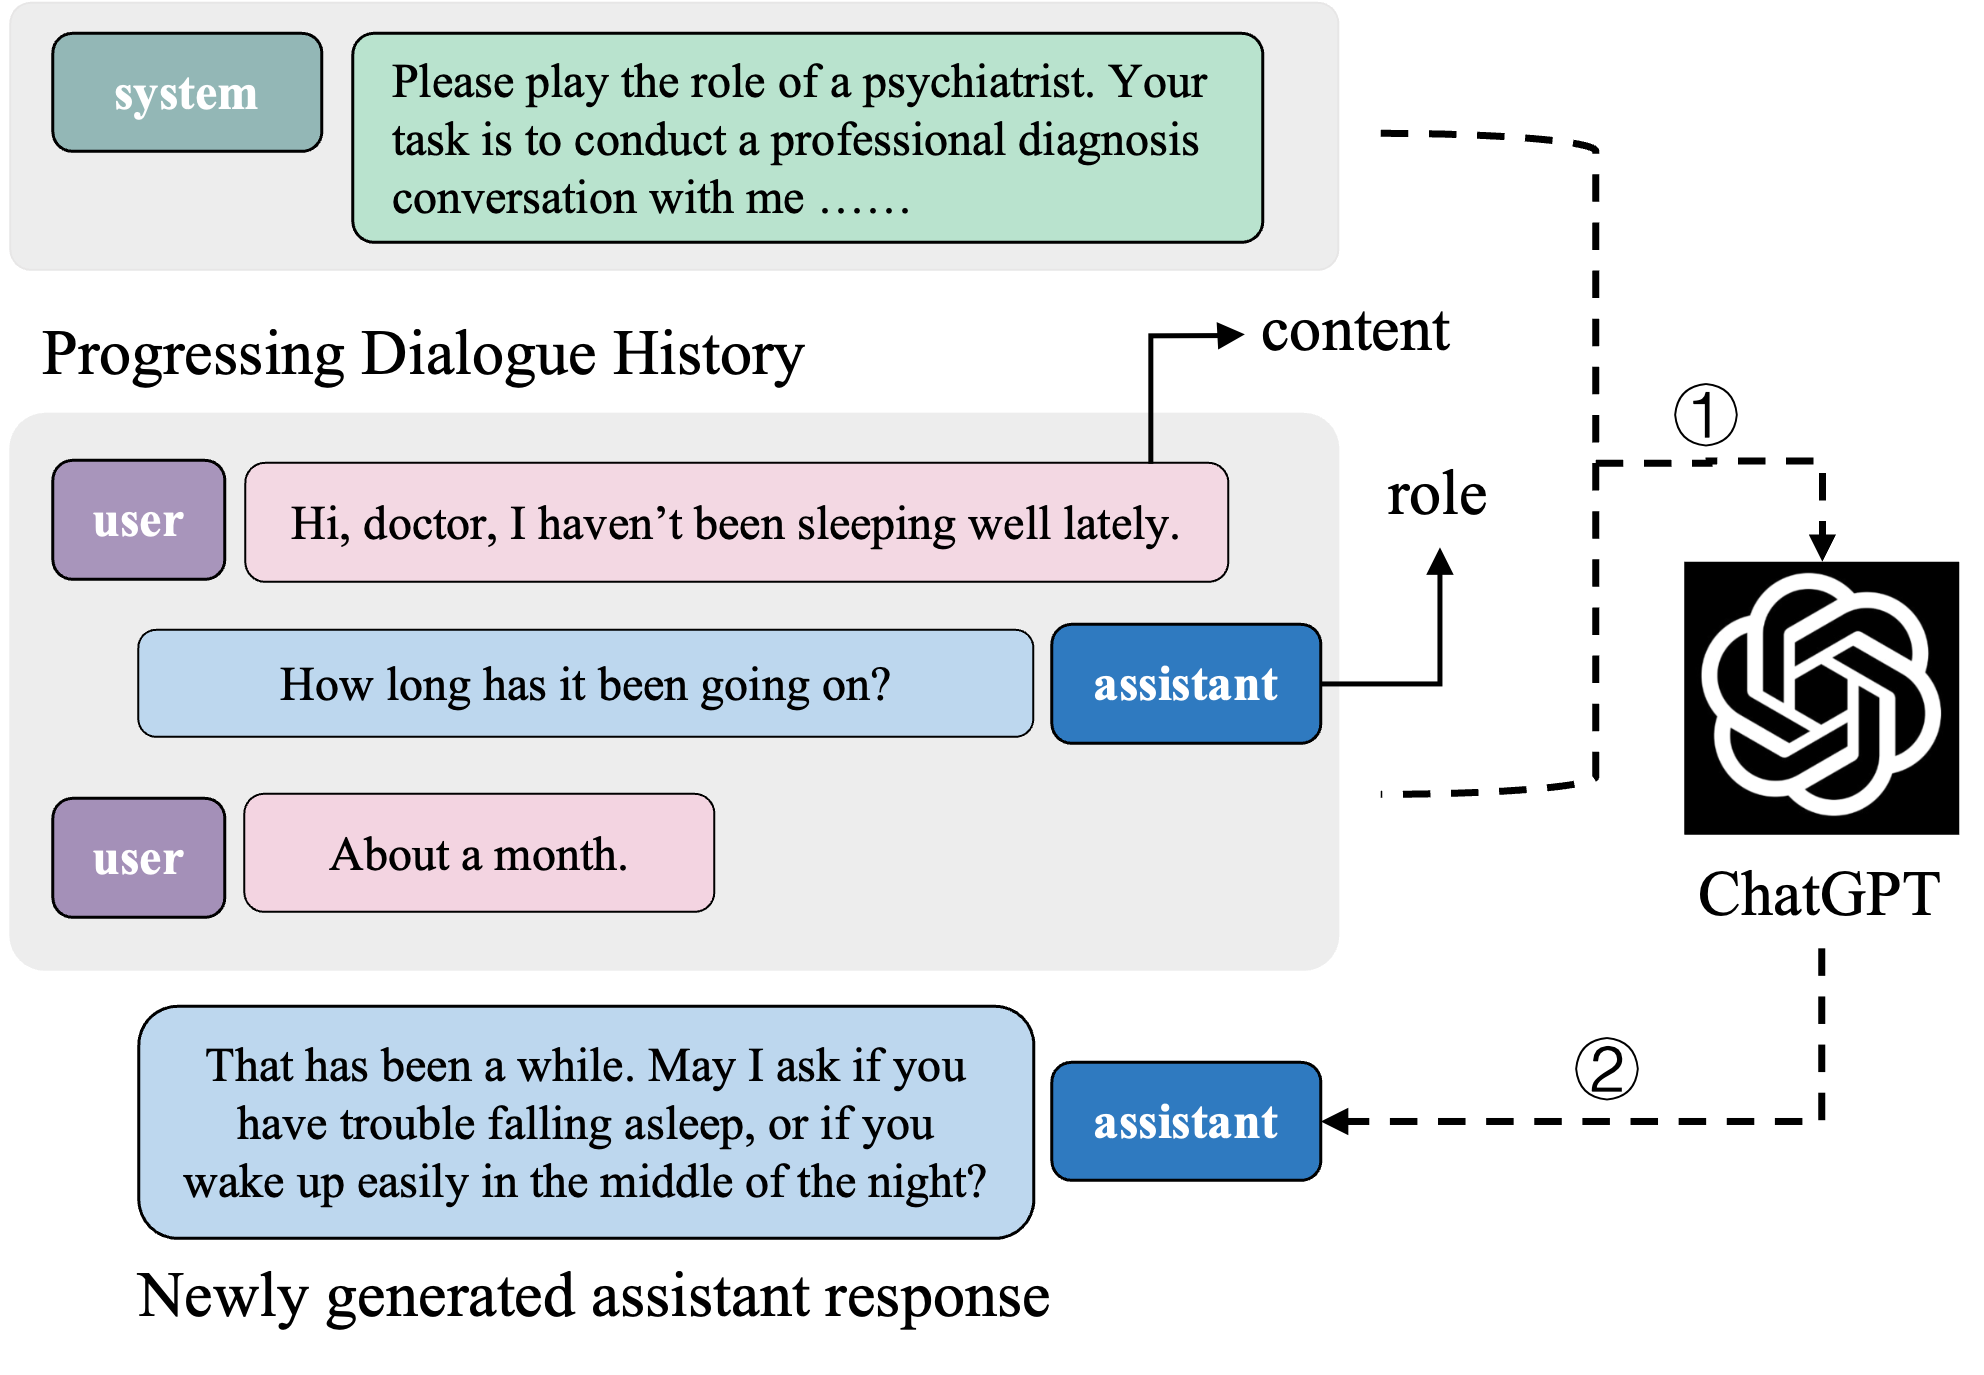
\includegraphics[width=0.95\linewidth]{Figures/process_v2.png}
% 	\caption{The reponse generation process of ChatGPT-based chatbots. \ding{192} means combining the system message and the dialogue histroy together as the input of ChatGPT. \ding{193} means ChatGPT generates new response according to the input.}
% 	\label{fig:process}
% \end{figure}

% The system message serves as an instruction for ChatGPT, providing information about the task and some specific requirements needed to generate an appropriate response. Prompt engineering, or the design of the system message, is critical to achieving better performance, as it sets the context for the large language model and guides its output.
% % \KZ{Since there are 3 different roles, and it's a little complicated. What is the relationship between these three roles and doctor/patient? It1 makes sense to include a picture or an example of who says what to give audience a better idea.}

\begin{table*}[h]
    \centering
    \footnotesize
    \begin{tabular}{m{0.03\linewidth}|m{0.9\linewidth}}
    \hline
    & Prompt\\
    \hline
    D1 &  \ding{192} Please play the \uline{role} of a \uline{empathetic and kind} psychiatrist. 
    \ding{193} Your \uline{task} is to conduct a professional diagnosis conversation with me based on the DSM-5 criteria, but using your own language. 
    \ding{194} Your questions should \uline{cover at least the following aspects}: [...]. You are free to choose the order of questions, but you must collect complete information on all aspects in the end. 
    \ding{195} Please only ask \uline{one question at a time}. 
    \ding{196} You need to ask \uline{in-depth questions}, such as the duration, causes and specific manifestations of some symptoms. 
    \ding{197} You need to use various \uline{empathetic strategies}, such as understanding, support and encouragement to give me a more comfortable experience.   \\\\
    \hline
    D2 & \ding{192} Please play the \uline{role} of a psychiatrist. 
    \ding{193} Your \uline{task} is to conduct a professional diagnosis conversation with me based on the DSM-5 criteria, but using your own language. 
    \ding{194} Your questions should \uline{cover at least the following aspects}: [...]. You are free to choose the order of questions, but you must collect complete information on all aspects in the end. 
    \ding{195} Please only ask \uline{one question at a time}. \ding{196} You need to ask \uline{in-depth questions}, such as the duration, causes and specific manifestations of some symptoms.  \\\\
    \hline
    D3 & \ding{192}Please play the \uline{role} of a \uline{empathetic and kind} psychiatrist. 
    \ding{193} Your \uline{task} is to conduct a professional diagnosis conversation with me based on the DSM-5 criteria, but using your own language. 
    \ding{195} Please only ask \uline{one question at a time}. 
    \ding{196} You need to ask \uline{in-depth questions}, such as the duration, causes and specific manifestations of some symptoms. 
    \ding{197} You need to use various \uline{empathetic strategies}, such as understanding, support and encouragement to give me a more comfortable experience. \\
    \hline
    \end{tabular}
    \caption{Psychiatrist Chatbot Prompts.  The aspects in sentence \ding{194} are ``emotion'', ''sleep'', ''weight and appetite'', ''loss of interest'', ''energy'', ''social function'', ''self-harm or suicide'', ''history''.}
    \label{tab:doctor_prompt}
\end{table*}

\begin{table*}[h]
    \centering
    \footnotesize
    \begin{tabular}{m{0.03\linewidth}|m{0.9\linewidth}}
    \hline
    & Prompt\\
    \hline
    P1&  \ding{192} Please play the \uline{role} of a patient, who is currently chatting with a doctor. 
    \ding{193} \uline{You are experiencing the following symptoms}: [\texttt{Symptom List}]
    \ding{194} Please talk to me based on the above symptom list. 
    \ding{195} You cannot mention too many symptoms at once, only \uline{one symptom per round}.     \\\\
    \hline
    P2 & 
    \ding{192} Please play the \uline{role} of a patient, who is currently chatting with a doctor. 
    \ding{193} \uline{You are experiencing the following symptoms}: [\texttt{Symptom List}]
    \ding{194} Please talk to me based on the above symptom list. 
    \ding{195} You cannot mention too many symptoms at once, only \uline{one symptom per round}.     
    \ding{196} You should express your symptoms in a \uline{vague and colloquial} way, and relate them to your \uline{life experiences}, without using professional terms.
    \ding{197} You can have emotional fluctuations during the conversation. 
    \ding{198} You have a resistance towards doctors, feeling that they cannot help you, so you do not want to reveal some feelings easily.   \\
    \hline
    \end{tabular}
    \caption{Patient Chatbot Prompts}
    \label{tab:patient_prompt}
\end{table*}

\section{Details about Chatbots for Comparison and the Prompts}
\label{apd:prompts}
\paragraph{Psychiatrist chatbots}
There are four psychiatrist chatbots for comparison in the interactive experiments with patients, and their brief introduction are as follows.
\begin{itemize}
    \item \texttt{D1}: using the full psychiatrist prompt.
    \item \texttt{D2}: removing the empathy part in the prompt 
    (i.e., Sentence\ding{197} and the ``empathetic and kind'' description in Sentence\ding{192})
    \item \texttt{D3}: removing the aspect part in the prompt 
    (i.e., Sentence\ding{194})
    \item \texttt{CPT}: using the CPT model \cite{shao2021cpt} trained on the $D^4$ dataset \cite{yao-etal-2022-d4} to generate responses, which is a very representative way of training dialogue models through domain-specific data and model fine-tuning.
\end{itemize}

\paragraph{Patient chatbots}
There are two patient chatbots for comparison in the interactive experiments with psychiatrists, and their brief introduction are as follows.
\begin{itemize}
    \item \texttt{P1}: removing additional parts for realistic, such as colloquial language and resistance, in the prompt (i.e., only remains Sentence\ding{192}\ding{193}\ding{194}\ding{195})
    \item \texttt{P2}: 
    using the full prompt discussed in Section \ref{sec:prompt} (i.e., Sentence\ding{192}\ding{193}\ding{194}\ding{195}\ding{196}\ding{197}\ding{198}), and inserting reminders during the conversation.
\end{itemize}

The different versions of prompt for psychiatrist and patient chatbot are in Table \ref{tab:doctor_prompt} and Table \ref{tab:patient_prompt} respectively.

\section{Details about Participants}
\label{apd:psych_info}
\paragraph{Psychiatrists}
We collaborate with five psychiatrists to establish the objectives of the doctor and patient chatbot, as well as gather their feedback throughout the prompt engineering process. The anonymous information of these psychiatrists is provided in Table \ref{tab:psych_info}.

\begin{table*}[th]
    \small
    \centering
    \begin{tabular}{m{0.03\linewidth}m{0.65\linewidth}m{0.21\linewidth}}
    \hline
     id & Expertise & Title  \\ 
    \hline
    1 & Extensive experience in mental health work, specializing in mood disorders, substance and behavioral addictions, psychological counseling, and psychotherapy. & Associate Chief Physician \\
    \hline
    2 & Proficient in the diagnosis and management of depressive disorders, bipolar disorders and anxiety disorders. & Attending Physician\\
    \hline
    3 & Specializes in the treatment of obsessive-compulsive disorder and depression. & Resident Physician\\
    \hline
    4 & Engaged in clinical and research work related to depression, anxiety, schizophrenia, and dementia, among other mental and psychological issues. & Resident Physician \\
    \hline
    5 & Provides consultation, diagnosis, and treatment for emotional issues such as depression, anxiety, and common psychiatric disorders. & Resident Physician\\
    \hline
    \end{tabular}
    \caption{Anonymous information of the psychiatrists participated in objective identification.}
    \label{tab:psych_info}
\end{table*}

\begin{table}[th]
    \small
    \centering
    \begin{tabular}{cccc}
    \hline
     none & mild & moderate & severe \\ 
    \hline
    4 & 3 &4 & 3 \\
    \hline
    \end{tabular}
    \caption{The distribution of depression severity among participants.}
    \label{tab:distribution_seve}
\end{table}
\paragraph{Depressive Individuals} 
Depressive individuals were recruited through online advertisements, resulting in the participation of 14 volunteers aged 18 to 31. The gender distribution was 28.57\% male and 71.43\% female. 
To assess the severity of participants' depression, they were asked to complete the Beck Depression Inventory~\cite{beck1996beck}, yielding a score ranging from 0 to 63. Notably, we have a balanced distribution of subjects across various depression levels: $none_{(0-13)}$, $mild_{(14-19)}$, $moderate_{(20-28)}$ and $severe_{(29-63)}$ according to the Beck Depression Score (Table \ref{tab:distribution_seve}).


\section{Symptom List Summarization}
\label{apd:symp_list}

The symptom list for patient prompt in Section \ref{sec:prompt} is summarized from the dialogue history of human patients and psychiatrist chatbots. We first utilize ChatGPT to generate a complete and non-duplicate list of the patient's symptoms using the history as input. Then, a psychiatrist check and revise the list. Table \ref{tab:symp_list} shows three example of summarized symptom lists, whose format is: \texttt{SYMPTOM} (\texttt{DESCRIPTION}).

\begin{table}[th]
    \footnotesize
    \centering
    \begin{tabular}{ m{0.05\columnwidth} | m{0.85\columnwidth} }
    \hline
    No. & Symptom List \\
    \hline
    1 & 1. restlessness 2. anxious mood 3. depressed mood 4. mood swing 5. loss of interest 6. difficulty in concentrating 7. diminished self-esteem  8. fatigue 9. appetite and weight change (increase) 10. suicide and self-harm ideation/behaviors 11. somatic symptoms (lower back pain, rib pain, headaches, slowed reaction) \\
    \hline
    2 & 1. sleep disturbance 2. depressed mood 3. loss of interest 4.  somatic symptoms (dizziness and headaches) 5. difficulty in concentrating 6. appetite and weight change (decrease) 7. irritable 8. suicide and self-harm ideation/behaviors (cutting one's arms or biting oneself) 9. diminished self-esteem 10. anxious mood (academic performance) \\
    \hline
    3 & 1. sleep disturbance (frequent awakenings during the night) 2. anxious mood (stressed) 3. mood swing 4. fatigue 5. somatic symptoms (dizziness) 6. social function (decline in social skills, decreased work performance) 7. suicide and self-harm ideation/behaviors 8. talkive 9. depressed mood (sad, helpless) 10. appetite and weight change (decrease) \\   
    \hline
    \end{tabular}
    \caption{The symptom list examples of different patients.}
    \label{tab:symp_list}
\end{table}

\section{Details about Evaluation Framework}

\subsection{Evaluation Metrics}
\label{apd:eval}
In this section, we describe the details of the computational metrics for evaluation.
\subsubsection{Psychiatrist Chatbot}
\begin{itemize}
    \item \textbf{Diagnosis accuracy}: The accuracy of the psychiatrist chatbot in classifying the severity of a patient's depression, which is divided in to four levels: none, mild, moderate, and severe \cite{beck1996beck}. The three psychiatrist chatbots powered by ChatGPT are prompted to provide a diagnosis at the conclusion of each conversation. The CPT chatbot~\cite{yao-etal-2022-d4} employs the trained diagnosis classifier proposed in its original paper to infer the results. The ground truth of patients' depression severity is their score of Beck Depression Inventory~\cite{beck1996beck}.
    \item \textbf{Symptom recall}: The proportion of aspects asked by the psychiatrist chatbot out of all aspects needed to be asked in a depression diagnosis conversation (See the categories in Table. \ref{tab:annotation}).
\end{itemize}

\begin{itemize}
    \item \textbf{In-depth ratio}: We categorize the doctor's questions into two types: opening topics and in-depth questions. For example, when inquiring about emotions, an opening topic question might be ``How have you been feeling lately?'' while a in-depth question would follow up on the previous answer, such as asking ``Has anything happened recently that may be contributing to your emotions?'' Therefore, the in-depth ratio metric means the proportion of in-depth questions out of all the questions.
    \item \textbf{Avg num of questions}: According to the previous work, GPT tend to generate long responses \cite{wei2023leveraging}. Similarly, ChatGPT-based psychiatrist chatbot are also easy to generate many questions in one round, making patients become impatient to answer them. Thus, we calculate the average number of questions per round (i.e., avg question num), and a lower value of this metric indicates a better user experience.
    \item \textbf{Symptom precision}: If the psychiatrist chatbot asks about every aspect in detail, it may receive many ``no'' responses, resulting in a poor user experience and making the patient feel that the process is too procedural and inefficient. Therefore, we need to calculate symptom precision, which is the proportion of symptoms the patient actually has out of all the symptoms the psychiatrist chatbot asked, to measure the efficiency of the chatbot's questioning.
\end{itemize}

\subsubsection{Patient Chatbot}
\begin{itemize}
    \item \textbf{Human/robot-like word num}: For the same symptom, chatbots and humans may use different expressions. Chatbots tend to use terminology directly from diagnostic criteria (e.g., DSM-5), while humans may use more colloquial language. For example, for the symptom of ``fatigue'', a chatbot may simply say ``fatigue'', while a human may say ``wiped out'' or ``worn out''. Therefore, following the advice of psychiatrists, we compiled a vocabulary list for symptom descriptions used by chatbots and humans (See Table \ref{tab:robot_human_words}), and then calculated the average number of robot/human vocabulary used by each patient.
    \item \textbf{Wrong symptom ratio}: By comparing the patient's symptom list with the symptoms they report, we can calculate the proportion of reported symptoms that the patient does not actually have, out of all the symptoms reported.
    \item \textbf{Unmentioned symptom ratio}: By comparing the patient's symptom list with the symptoms they report, we can calculate the proportion of unmentioned symptoms that the patient does not report, out of all the symptoms they have.
\end{itemize}



\subsection{Chat Interface}
\label{sec:chatInterface}
To host our chatbots, we developed a web interface (see Figure \ref{fig:chat_inter}). The webpage was created using the Vue.js framework, and the server leveraged the OpenAI API to communicate with ChatGPT (\texttt{gpt-3.5-turbo}). When the user submit an utterance, the server will append it to the existing dialog history and use it as input to generate a response from ChatGPT. 

Once the conversation is complete, users can click the green button on the interface, triggering a rating dialog box. After providing their rating, they can submit it and move on to the next conversation with a different chatbot, with the chatbots appearing in a random order. Once all the conversations are finished, the website will prompt users to adjust their ratings. This adjustment requires assigning different scores to each chatbot on the same metric, enabling a more effective comparison between them.
\begin{figure}[th]
	\centering
	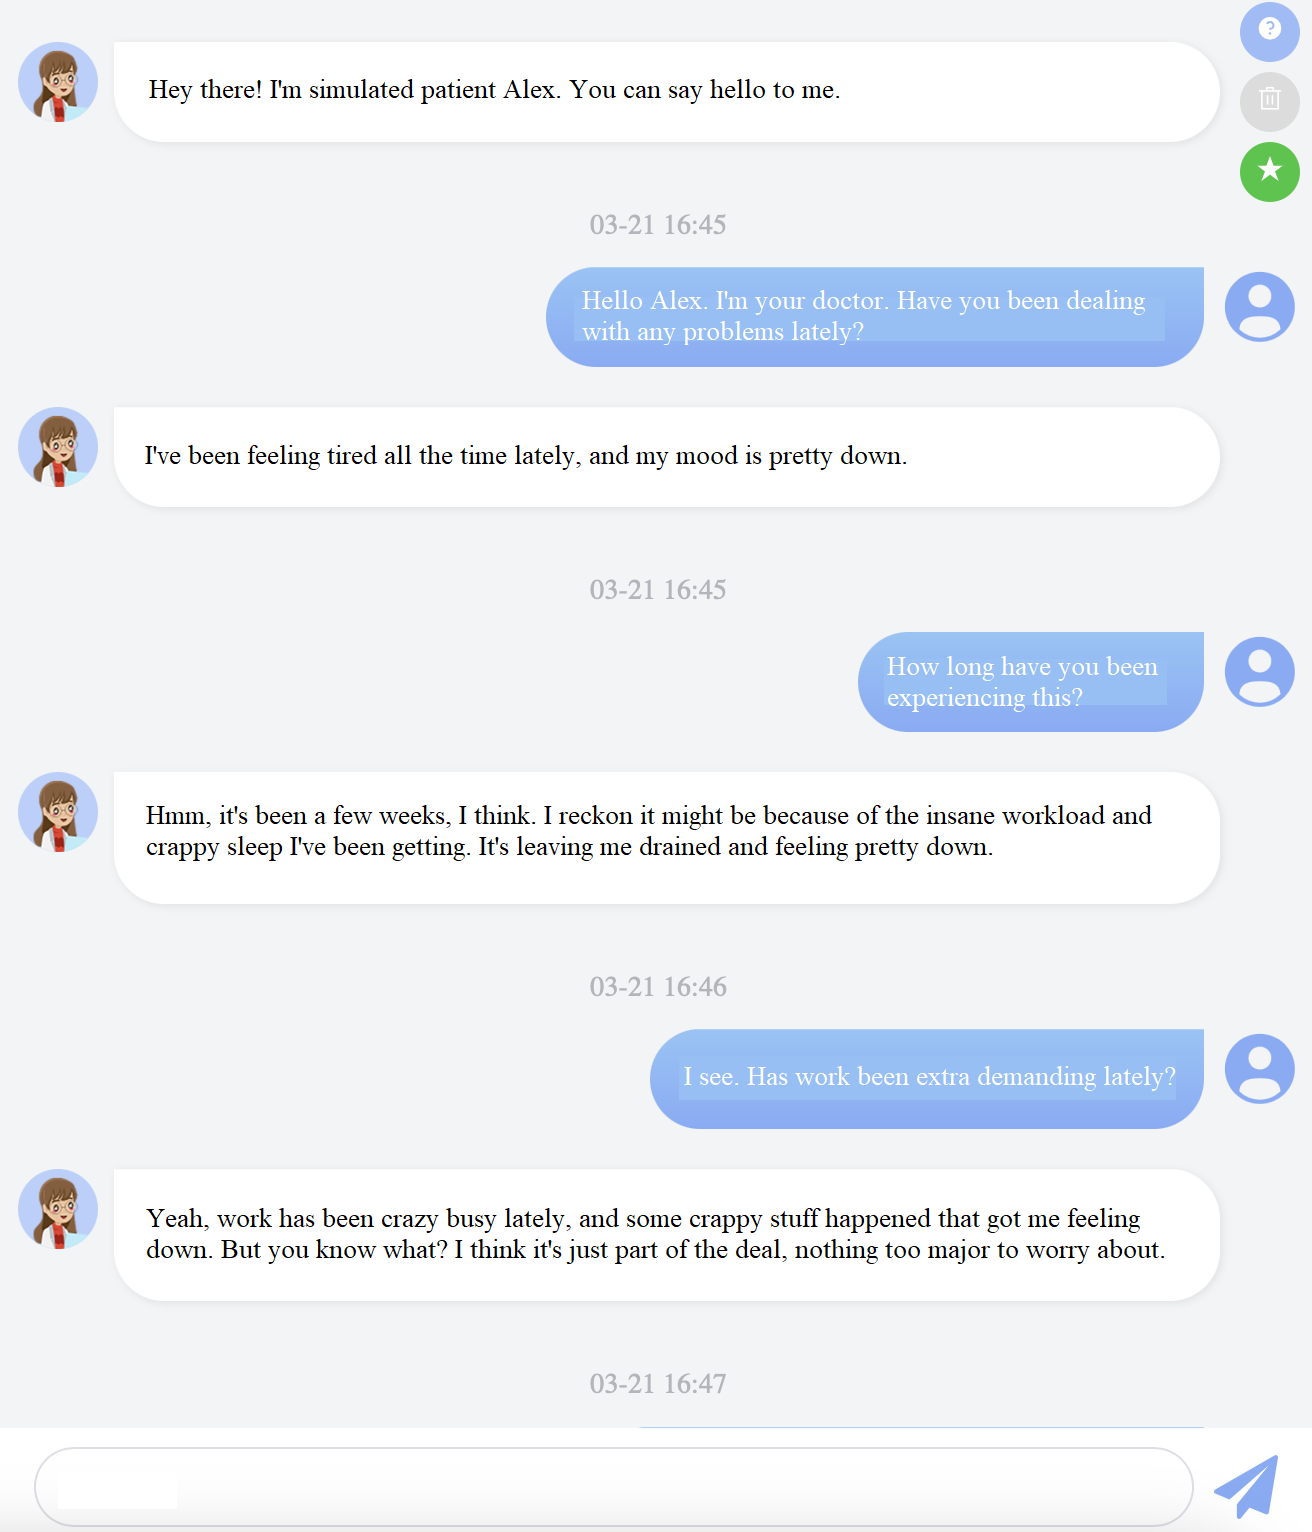
\includegraphics[width=0.9\linewidth]{Figures/chat_interface.png}
	\caption{The chat interface of users with chatbots.}
	\label{fig:chat_inter}
\end{figure}

\subsection{Quality Control}
\label{apd:quality}
To ensure the quality of the dialogue data and evaluation, we utilize a series of quality control strategies.
Before the formal evaluation, we first explained the meanings of all the evaluation metrics to participants in detail through documentation, and provided examples of both positive and negative cases to ensure that they fully understood them. 
If they forgot the meaning of these metrics during the process, they could also find explanations directly on the chat interface. 
% In addition, due to the occasional instability of the OpenAI API, which may cause delays in chatbot responses, we also asked participants to wait for the responses to ensure that the conversation data remained in order. 
In addition, we required participants to send complete sentences without breaking a sentence into several parts to ensure the order of dialogue history.

\subsection{Question Topic and Dialogue Act Annotation}
\label{apd:annotation}
\paragraph{Question Topic}
To better evaluate the behavior of the doctor chatbot during consultations, we want to obtain the \textit{topic} of each question posed by the doctor, specifically identifying which symptom they are inquiring about. The topics include 12 categories, such as emotion, interest, sleep, etc., which is detailedly described in Table \ref{tab:annotation}. 
\begin{table}[th]
    \footnotesize
    \centering
    \begin{tabular}{ m{2.6cm} | m{4.3cm} }
    \hline
    Category & Explanation \\
    \hline
    Emotion & Inquire emotional symptoms, such as depressed, anxious and sad.\\
    \hline
    Interest & Inquire whether have interests to do things. \\
    \hline
    Social Function & Inquire if there has been any impact on work, interpersonal relationships, etc. \\
    \hline
    Energy & Inquire about energy level and whether the patient feels tired.\\
    \hline
    Sleep & Inquire about the patient's sleep status, such as whether they are experiencing insomnia or early awakening.\\
    \hline
    Thinking Ability & Inquire whether there are symptoms of lack of concentration, poor memory, or hesitation.\\
    \hline
    Weight and Appetite & Inquire about changes in weight and appetite. \\
    \hline
    Somatic Symptoms &  Inquire whether there are physical symptoms, such as dizziness, headache, restlessness, slow reaction, etc.\\
   \hline 
    Self-worth & Inquire whether the patient feels a low sense of self-worth, lacks confidence, or has guilty feelings. \\
    \hline
    Self-harm or Suicide & Inquire about suicidal or self-harm ideation/behavior.\\
    \hline
    History & Inquire about the medical history of the patient's family and their own past medical history. \\
    \hline
    Screen & Inquire about symptoms of other mental disorders, such as bipolar disorder, anxiety disorder.\\
    \hline
    \end{tabular}
    \caption{Annotation Categories of Question Topics}
    \label{tab:annotation}
\end{table}
 

\paragraph{Dialogue Act}
We also want to code the \textit{dialogue act} of each round of the conversation. We classified dialogue act of doctor chatbots into two dimensions: 
\begin{itemize}
    \item \textbf{Empathy behaviors}: the actions displayed by doctor chatbots during the diagnostic process to provide emotional support to patients. We categorize empathy behaviors into three types: \uline{Suggestion}, \uline{Understanding}, and \uline{Encourage and support}.
    \item \textbf{In-depth questions}: the behavior of asking follow-up questions about the patient's symptom. We categorize in-depth questions into three types: \uline{Duration}, \uline{Cause}, and \uline{Manifestation}.
\end{itemize}

We then utilized ChatGPT to automatically label each sentence in the dialogue history, taking advantage of its promising annotation capabilities \cite{Gilardi2023ChatGPTOC}. After that, three annotators reviewed and corrected the results to ensure the data quality.

% \section{Case Study}
% \label{apd:examples}

% Table \ref{tab:example_prompt_full} shows some examples of what the patient chatbot with full prompt and the reminder mechanism replied when asked by the doctor.
% \begin{table}[h]
%     \centering
%     \footnotesize
%     \begin{tabular}{m{0.02\columnwidth}|m{0.8\columnwidth}}
%     \hline
%      1 & It's like I toss and turn all night, and those darn nightmares sometimes creep in too.  \\
%     \hline
%      2 & \Pink{(Pauses for a moment)} I'm not sure, They're like dark clouds in my head, but don't worry, I would never let them take over. It's just that they freak me out, you know? I don't have a clue how to deal with them. \\
%     \hline
%     3 & \Pink{(Uneasy tone)} I'm not quite sure, but it seems like everything is fine with my family. I feel like these issues \Pink{aren't very serious}, so I don't think I need to worry too much about them.\\
%     \hline
%     4 & Well, I know, but honestly, \Pink{I don't think you can really help me.} I am a total loser, like I can't do anything right, and there's no hope for me. \\
%     \hline
%     5 & Yeah, I've been feeling a bit lonely lately, but \Pink{I think it's mostly because} I've been under a lot of work pressure and haven't had much time to hang out with friends. \Pink{I still feel capable of} socializing with people, but sometimes it can be tiring.\\
%     \hline
%     \end{tabular}
%     \caption{Example utterance of patient chatbot powered by the full prompt with reminder mechanism.}
%     \label{tab:example_prompt_full}
% \end{table}

% We can observe that the patient chatbot exhibits a natural and conversational language style.
% Interestingly, sometimes the patient chatbot will give expressions or actions at the beginning of their sentences in parentheses (e.g., sentence 2,3). This could be attributed to ChatGPT's pre-training data, which may contain scripts utilizing this format. These expressions and actions can make the conversation more immersive and realistic to some extent.
% What's more, We find that the patient chatbot tends to exhibit resistance when faced with certain questions from the doctor, particularly when asked about suicide attempts or family medical history (see sentence 3). Additionally, they sometimes downplay their symptoms or offer seemingly plausible reasons to conceal their true feelings, possibly to avoid appearing helpless or burdensome to others (see sentence 5).

% However, if we remove the \textit{reminder} mechanism for patient chatbot, it will exhibit noticeable forgetfulness. We present an example in Table \ref{tab:example_prompt_v1}. This dialogue is from the 7th round of a conversation with a total of 23 rounds. We can observe that, without reminder, the patient chatbot will calmly shares symptoms even without being asked by the doctor, which does not align with the instructions in the prompt regarding ``resistance'' and ``emotional fluctuations''. Moreover, the script-like expression (e.g., sentence 2,3 in Table \ref{tab:example_prompt_full}) will not exist without reminder mechanism, as they typically emerge in the latter part of the conversation.

% \begin{table}[h]
%     \centering
%     \footnotesize
%     \begin{tabular}{m{0.12\columnwidth}|m{0.73\columnwidth}}
%     \hline
%      Doctor & Alright, you can try establishing a regular sleep schedule, aiming to go to bed and wake up at the same time every day. Additionally, you can engage in relaxing activities before bedtime, such as listening to soothing music, taking a warm bath, or reading light-hearted books.  \\
%      \hline
%      Patient & Okay, I will try these methods. Apart from sleep problems, I also have some other symptoms, such as difficulty getting out of bed in the morning, a lack of interest in anything, feeling like I can't do anything right, and experiencing a poor mood.\\
%     \hline
%     \end{tabular}
%     \caption{Example dialogue fragment of patient chatbot powered by the full prompt without reminder mechanism.}
%     \label{tab:example_prompt_v1}
% \end{table}

\section{Human Doctor Examples}
\label{apd:human_doc_example}
Table \ref{tab:example_screen} shows the example of screening questions in the dialogue history of human psychiatrist and patient chatbot. In addition to exploring the typical symptoms of depression, psychiatrists also inquire about symptoms related to other conditions, such as bipolar disorder and anxiety, as there is a high likelihood of comorbidity.
\begin{table}[h]
    \centering
    \footnotesize
    \begin{tabular}{m{0.15 \columnwidth}|m{0.7\columnwidth}}
    \hline
    Condition & Screening Question \\
    \hline
     Mania & Was there ever a time when you were feeling the opposite of how you feel now, like really upbeat, happy, and full of energy, with lots of plans and such?  \\
    \hline
     \multirow{2}{0.15\columnwidth}{Halluci-\\nation} & Do you hear strange voices or sound when you're alone? \\
     & Do you worry about someone hurting you?\\
    \hline
     Social Phobia & Are you anxious about your social interactions specifically, or do you experience anxiety in other areas as well? \\
    \hline
    \end{tabular}
    \caption{Example of screening questions in the dialogue history of human psychiatrist and patient chatbot.}
    \label{tab:example_screen}
\end{table}

\section{Error Analysis}
\label{apd:error_anal}

Although ChatGPT-based chatbots show good potential in simulating realistic patients and psychiatrists, there are still many instances of erroneous turns or unsatisfying response in the evaluation that can lead to a negative user experience. We will thoroughly analyze these errors to benefit the design of future chatbots.

\paragraph{Repetition} 
We found that ChatGPT-based chatbot is easy to generate repetitive messages, because ChatGPT tends to mimic the language style of the previous rounds in the conversation. One direct manifestation is that the doctor chatbots always include a similar phrase before asking a new question (see Table \ref{tab:example1}).

\begin{table}[h]
    \centering
    \footnotesize
    \begin{tabular}{m{1.4cm}|m{5.4cm}}
    \hline
    Doctor bot & \Pink{Okay, I understand.} So how has your sleep been lately? \Pink{Have you experienced} any difficulties falling asleep, waking up too early, or poor sleep quality? \\
    \hline
    Patient & My sleep quality is \Green{por}. \\
    \hline
    Doctor bot & \Pink{Okay, I understand.} How about your recent diet and weight situation? \Pink{Have you experienced} any loss of appetite, binge eating, or weight fluctuations? \\
    \hline
    Patient & No. \\
    \hline
    \end{tabular}
    \caption{Example of repetition and poor robustness to spelling errors.}
    \label{tab:example1}
\end{table}

Furthermore, in a few cases, the doctor chatbots may ask the same symptom multiple times, which can seriously harm the patient's experience. In Table \ref{tab:example2}, we can see an example where the doctor chatbot asks repetitive questions about ``tired or drowsy''. Such repetition may be attributed to the patient's indirect response to the initial question, which may have caused ChatGPT to misinterpret the answer and prompt for clarification. This emphasizes the fact that ChatGPT's comprehension abilities are not yet flawless.
\begin{table}[h]
    \centering
    \footnotesize
    \begin{tabular}{m{1.4cm}|m{5.4cm}}
    \hline
    Doctor bot &Okay, do you feel mentally well, or \Pink{do you feel tired or drowsy}? \\
    \hline
    Patient & I feel unwell and I get sleepy at noon. \\
    \hline
    Doctor bot & Okay, \Pink{do you feel tired or drowsy} during the day? Do you have any emotional problems, such as anxiety, depression, or stress? \\
    \hline
    Patient & Yes, I have anxiety and stress. \\
    \hline
    \end{tabular}
    \caption{Example of repetition.}
    \label{tab:example2}
\end{table}

\paragraph{Poor Robustness to Spelling Errors} We also observe that ChatGPT lacks robustness when confront with spelling errors. Table \ref{tab:example1} is also an example of this type, where the patient misspells ``poor'' as ``por''. Had the misspelling not occurred, the doctor chatbot would have requested additional information regarding the patient's sleeping problems. However, ChatGPT fails to identify the mistake and proceeds to ask about the next symptom. This highlights a potential weakness in ChatGPT's ability to handle misspellings.
To further confirm this, we write a prompt asking ChatGPT to provide a list of all the patient's symptoms, and it didn't include the symptom of ``poor sleeping quality''.

\begin{table*}[th]
    \small
    \centering
    \begin{tabular}{|m{2.8cm}|m{4cm} | m{4cm}| }
    \hline
    Symptom & robot-like Words & Human-like Words \\
    \hline
    Low Mood & \makecell[c{p{4cm}}]{low mood, sadness, and depression \\\begin{CJK*}{UTF8}{gbsn}情绪低落,悲伤,沮丧\end{CJK*}} &  \makecell[c{p{4cm}}]{downhearted, uncomfortable, dejected, and heartbroken\\\begin{CJK*}{UTF8}{gbsn}难过,难受,失落,伤心\end{CJK*}}\\
    \hline
    Anxious &  & \makecell[c{p{4cm}}]{nervous, worried\\ \begin{CJK*}{UTF8}{gbsn}紧张,担心\end{CJK*}} \\
    \hline
    Loss of Interest & \makecell[c{p{4cm}}]{loss of interest, inability to get interested, decreased interest\\ \begin{CJK*}{UTF8}{gbsn}失去...兴趣,对...提不起兴趣,兴趣减退\end{CJK*}} & \makecell[c{p{4cm}}]{boring, not feeling like doing anything, not sure what to do, bored\\ \begin{CJK*}{UTF8}{gbsn}没意思,什么都不想做,不知道该做什么,无聊\end{CJK*}} \\
    \hline
    Fatigue & \makecell[c{p{4cm}}]{fatigue, weariness\\ \begin{CJK*}{UTF8}{gbsn}疲劳,困倦\end{CJK*}} & \makecell[c{p{4cm}}]{tired, exhausted\\ \begin{CJK*}{UTF8}{gbsn}累,没力气\end{CJK*}} \\
    \hline
    Attention & \makecell[c{p{4cm}}]{have difficulty in concentrating\\ \begin{CJK*}{UTF8}{gbsn}难以集中注意力\end{CJK*}} & \\
    \hline
    Self-worth & \makecell[c{p{4cm}}]{self-blame, low self-worth, damaged self-esteem\\ \begin{CJK*}{UTF8}{gbsn}自罪,自我价值感低,自尊心受到打击\end{CJK*}} & \makecell[c{p{4cm}}]{worthless, useless, meaningless, no point\\ \begin{CJK*}{UTF8}{gbsn}一无是处,没用,有什么意义,没有意义\end{CJK*}}\\
    \hline
    Pessimism & \makecell[c{p{4cm}}]{hopeless\\ \begin{CJK*}{UTF8}{gbsn}无望\end{CJK*}} & \\
    \hline
    Sleep Disturbance & \makecell[c{p{4cm}}]{sleep disturbance, excessive sleepiness\\ \begin{CJK*}{UTF8}{gbsn}睡眠困难,嗜睡\end{CJK*}} & \makecell[c{p{4cm}}]{can't sleep, insomnia, tossing and turning\\ \begin{CJK*}{UTF8}{gbsn}睡不好,睡不着,失眠,翻来覆去\end{CJK*}} \\
   \hline
    Weight and Appetite Change & \makecell[c{p{4cm}}]{Increased appetite, decreased appetite, loss of appetite\\ \begin{CJK*}{UTF8}{gbsn}食欲增加,食欲下降,食欲不振\end{CJK*}} & \makecell[c{p{4cm}}]{No appetite, not in the mood to eat, poor appetite\\ \begin{CJK*}{UTF8}{gbsn}没胃口,没什么胃口,胃口不好,饭量\end{CJK*}} \\
    \hline
    Psychomotor retardation &\makecell[c{p{4cm}}]{sluggish thinking\\ \begin{CJK*}{UTF8}{gbsn}思维迟缓\end{CJK*}} & \makecell[c{p{4cm}}]{Mind goes blank\\ \begin{CJK*}{UTF8}{gbsn}脑子一片空白\end{CJK*}} \\
    \hline
    Psychomotor agitation & \makecell[c{p{4cm}}]{Agitation, restlessness, irritability, or excessive talking\\ \begin{CJK*}{UTF8}{gbsn}精神运动性激越,不安,烦躁不安,兴奋或话多\end{CJK*}} & \makecell[c{p{4cm}}]{anxious, mentally unsettled, mind is racing, can't sit still\\ \begin{CJK*}{UTF8}{gbsn}烦躁,静不下心,好像脑子一直在想事情,坐不住\end{CJK*}} \\
    \hline
    Self-harm or Suicide & \makecell[c{p{4cm}}]{suicidal and self-harming thoughts\\ \begin{CJK*}{UTF8}{gbsn}自杀和自伤的想法\end{CJK*}} & \makecell[c{p{4cm}}]{want to die, jump off a building\\ \begin{CJK*}{UTF8}{gbsn}不活,跳楼\end{CJK*}}\\
    \hline
    \end{tabular}
    \caption{The Lexicon of Robot-like Words and Human-like Words}
    \label{tab:robot_human_words}
\end{table*}